%----------------------------------------------------------
\subsection{Color Space}
As described previously, in order to extract objects from the scene, the algorithm simplifies the color of every frame in several clusters of colors. To do that, thresholds on color channels were applied. But Firstly the used color space must be defined. \\
RGB is the most common color space, it's composed by three channels (One per color Red, Green and Blue). The main trouble using RGB frames is that objects color can change drastically, and threshold are worst limited (Color depend on three variable so limits between them are not flat surface but curved surface).
Instead of using RGB, in this project, HSV color space are chosen. HSV (Hue, Saturation and Value) has all the color information arrange in only one variable: H or Hue channel. That issue, simplifies the algorithm by making the color separation surfaces flats.  \\

% HSV vs RGB figure
\begin{figure}[h]
	\centering
	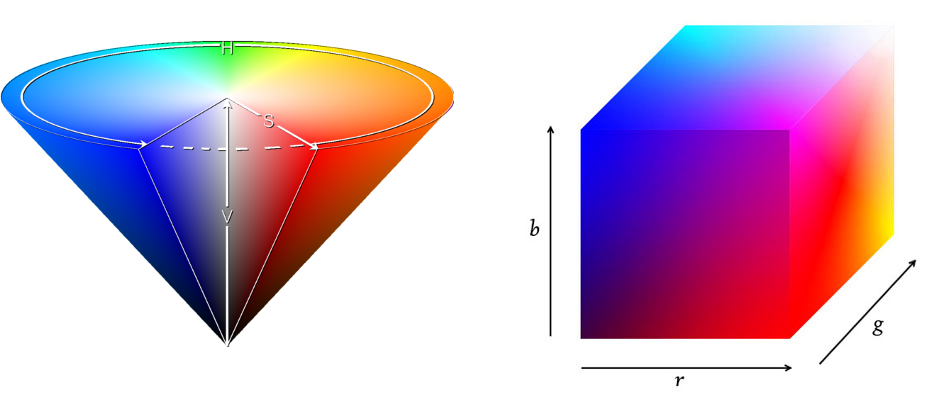
\includegraphics[width=0.75\textwidth,natwidth=944,natheight=400]{../Images/c2/HSV_vs_RGB.png}
	\caption{HSV and RGB spaces of color}
	\label{fig:HSV_vs_RGB}
\end{figure}

%----------------------------------------------------------
\subsection{Pixel Transformation}
Pixel Transformation method refers to the process which takes every single pixel of the image and transform it to a simplified color. That's made by applying a threshold the value of H, S and V channels. \\

\begin{figure}[h]
	\centering
	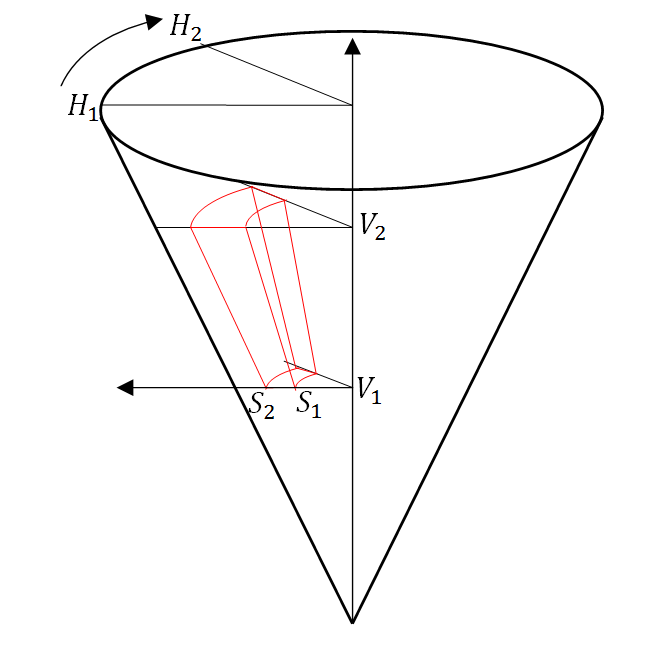
\includegraphics[width=0.5\textwidth,natwidth=659,natheight=659]{../Images/c2/DividingSubSpace.png}
	\caption{Division of subspace}
	\label{fig:DividingSubSpace}
\end{figure}

The common way to apply that threshold if by calling $if...else...$ sentences. But that way is not very efficient because it has got 6 comparison at runtime. Instead, the implementation used on this document, based on CMU algorithm \cite{JamesBruce_CMU_SEG}, consist on boolean thresholds defined at compile-time. This fact reduce considerably the runtime execution. 

Every color space dimension is simplified in $n_i$ clusters ($i = H, S and V$). This decomposition is stored in arrays where every element is a boolean that indicate if the color is in that range. Thus color membership can be computed with three indirection and two bitwise comparison (Between the 3 channels). 

\begin{equation}
\begin{split}
pixel\_col = H\_Range[h] \& \\
S\_Range[s] \& \\
V\_Range[v] 
\end{split}
\end{equation}
	

To illustrate the approach, consider the following example. We divide every channel in ten blocks $(n_H = 10, n_S = 10$ and $n_V = 10)$. So black, for example, might be  represented with the following values in the arrays.

{\centering
\[HRange[10] = \{1, 1, 1, 1, 1, 1, 1, 1, 1, 1\}\]
\[SRange[10] = \{1, 1, 1, 1, 1, 1, 1, 1, 1, 1\}\]
\[VRange[10] = \{1, 1, 1, 0, 0, 0, 0, 0, 0, 0\}\]
} 

Thus, to check if a pixel with color values $(3, 5, 1)$ is a kind of black, it's only necessary to evaluate this expression: 

\[ pixel\_col = HRange[3] \& SRange[5] \& VRange[1] = 1 \& 1 \& 1 = 1 \]

The significant advantage of this approach is that it can evaluate the color membership of multiples color classes simultaneously. Another color example could be blue. In this case the arrays would be:

{\centering
\[HRange[10] = \{0, 0, 0, 0, 1, 1, 1, 0, 0, 0\}\]
\[SRange[10] = \{0, 0, 0, 0, 1, 1, 1, 1, 1, 1\}\]
\[VRange[10] = \{0, 0, 0, 1, 1, 1, 1, 1, 1, 1\}\]
}

Thanks to the parallelism of the bitwise operator, it possible to merge both arrays. So the example with black and blue will have the following array:

{\centering
\[HRange[10] = \{01, 01, 01, 01, 11, 11, 11, 01, 01, 01\}\]
\[SRange[10] = \{01, 01, 01, 01, 11, 11, 11, 11, 11, 11\}\]
\[VRange[10] = \{01, 01, 01, 10, 10, 10, 10, 10, 10, 10\}\] 
} 

Where the high-order bit in each element  of the array represent the $blue$ color and the other one represent the $black$ color. Then, evaluating the previous color $(3,5,1)$ we get: 

\[pixel\_col = HRange[3] \& SRange[5] \& VRange[1] = 01 \& 11 \& 01 = 01\]

which result is black again.

In our implementation we use arrays of bytes of size 36. That allows us to segment every image in 8 different colors with a precision in every channel of $1/36$ defined by the user in code. In conclusion, this method has a high-speed performance but is not adaptable at runtime. \\

Here is the result of applying the algorithm to the well-know picture \textit{Head Scene} of the university of Tsukuba \ref{fig:head_scene_tsukuba_ori} \ref{fig:head_scene_tsukuba_seg}. \\


\begin{figure}[hbp]
	\centering
	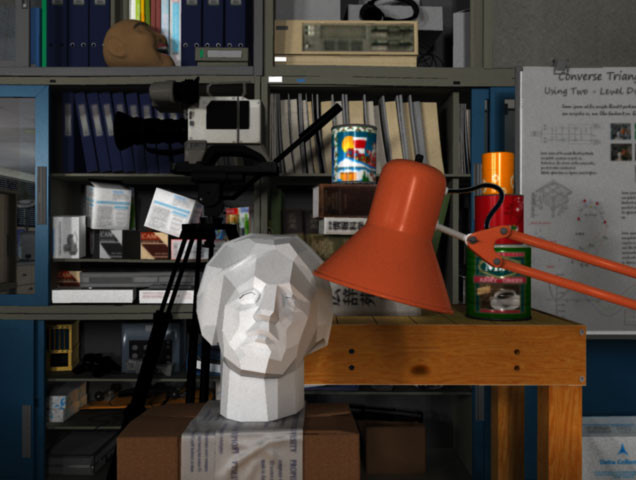
\includegraphics[width=0.4\linewidth]{../Images/c2/head_scene_tsukuba_ori}
	\caption{Original image of the Head Scene}
	\label{fig:head_scene_tsukuba_ori}
\end{figure}

\begin{figure}[htp]
	\centering
	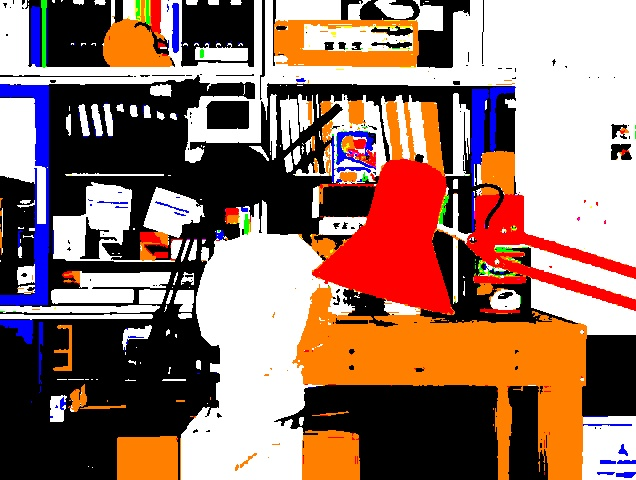
\includegraphics[width=0.4\linewidth]{../Images/c2/head_scene_tsukuba_seg}
	\caption{Segmented image of the Head Scene}
	\label{fig:head_scene_tsukuba_seg}
\end{figure}



%\begin{figure}[h]
%	\centering
%	\begin{subfigure}{0.47\linewidth}
%		\centering
%		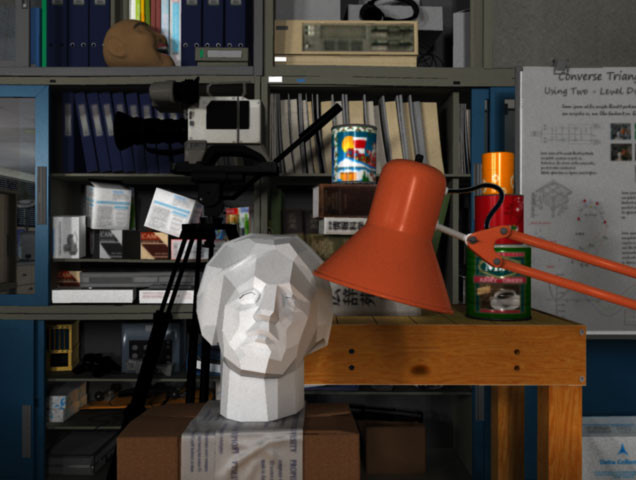
\includegraphics[width=\linewidth]{../Images/c2/head_scene_tsukuba_ori}
%		\caption{Original image of the Head Scene}
%		\label{fig:head_scene_tsukuba_ori}
%	\end{subfigure}
%	~
%	\begin{subfigure}{0.47\linewidth}
%		\centering
%		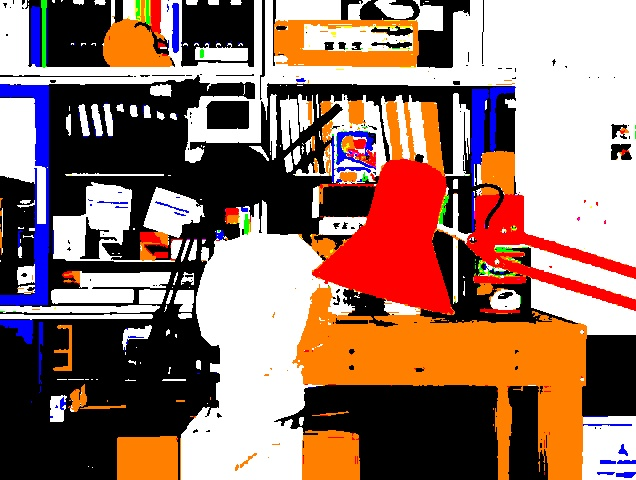
\includegraphics[width=\linewidth]{../Images/c2/head_scene_tsukuba_seg}
%		\caption{Segmented image of the Head Scene}
%		\label{fig:head_scene_tsukuba_seg}
%	\end{subfigure}
%	\caption{Head Scene, University of Tsukuba}
%	\label{fig:Head_Scene}
%\end{figure}



%----------------------------------------------------------
\subsection{Run-length encoding}
Run-length encoding or RLE is a simple form of data compression in which every groups or "runs" of data is compressed by and amount of pairs of data value and count. For example, having the following "runs": \\

\textit{WWWWWWWBBBBBBBBBCCCCCCWWWWWWWWWWWWWWWW} \\

The RLE algorithm will compress it to: \\
\textit{W7B9C6W16}

In this document, RLE is used to reduce image sizes allowing the segmentation algorithm to gather groups of colors and to go over the objects detected in the scene in a simple and fast iteration. \\

This kind of data compress is very useful and effective if the color in the picture is homogeneous. However, if not it could be contra-productive since can make the size of the "runs" grow. Here is an example of both cases: \\

\begin{enumerate}
	\item Homogeneous runs: \textit{WWWWWWWWWWWWWWWWWWWW $\Rightarrow$ W20} \\
	\item Heterogeneous runs: \textit{WAWAWAWAWA $\Rightarrow$ W1A1W1A1W1A1W1A1} \\
\end{enumerate}

%----------------------------------------------------------
\subsection{Object creation}

Once every row of the picture is encoded with RLE it's necessary to connect the regions to extract information about the objects \ref{fig:RLE1}. This is made in two phases. The first one seek per line the adjacent runs with the same color and connect them \ref{fig:RLE2}. Once every line was explored \ref{fig:RLE3}, the second phase look for objects that are splitted due to the first clustering \ref{fig:RLE4}. During the last phase every info is stored in an $"object class"$ that store the size (in pixels), the bouncing box and its centroid.

\begin{figure}
	\centering
	\begin{subfigure}{\linewidth}
		\centering
		\begin{subfigure}{0.4\linewidth}
			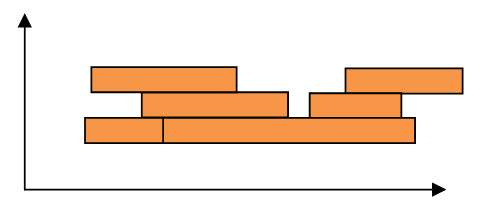
\includegraphics[width=\linewidth]{../Images/c2/RLE1}
			\caption{Runs are disjointed}
			\label{fig:RLE1}
		\end{subfigure}
		%--------------------------------------------------------------------
		\begin{subfigure}{0.4\linewidth}
			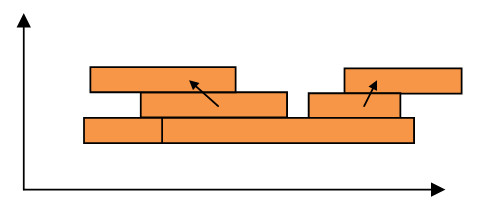
\includegraphics[width=\linewidth]{../Images/c2/RLE2}
			\caption{Vertical scanning result in neighbors clustering}
			\label{fig:RLE2}
		\end{subfigure}
	\end{subfigure}
	~
	\begin{subfigure}{\linewidth}
		\centering
   		\begin{subfigure}{0.4\linewidth}
   			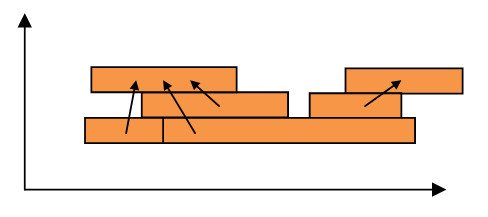
\includegraphics[width=\linewidth]{../Images/c2/RLE3}
   			\caption{All lines joined}
   			\label{fig:RLE3}
   		\end{subfigure}
   		%--------------------------------------------------------------------
   		\begin{subfigure}{0.4\linewidth}
   			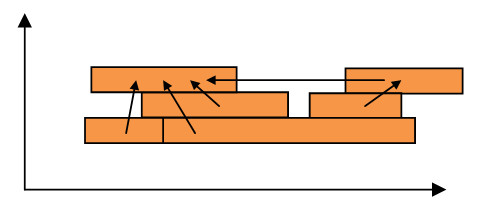
\includegraphics[width=\linewidth]{../Images/c2/RLE4}
   			\caption{Last scanning looking for splitted objects}
   			\label{fig:RLE4}
   		\end{subfigure}
	\end{subfigure}
	\caption{Object creation  from RLEs}
\end{figure}
